\documentclass[a4paper, 12pt]{article}

\usepackage{chirpstyle}

\begin{document}

\section*{2005 AIME I Solutions}

\begin{chirpbox}
\begin{problemnum}
    Six congruent circles form a ring with each circle externally tangent to two circles adjacent to it. All circles are internally tangent to a circle \( C \) with radius \( 30 \). Let \( K \) be the area of the region inside circle \( C \) and outside of the six circles in the ring. Find \( \lfloor K \rfloor \).
\end{problemnum}
\end{chirpbox}

\begin{solution}
    Our solution takes the form of
    \[
        K = 900\pi - 6 \pi r^2
    ,\]
    where \( r \) is the radius of one of the inner congruent circles. If one draws a diagram, this value is quite simple to solve for. Consider the triangle \( OAB \) in the diagram below. Let \( AB = r \) and observe that \( OB  = 30 - 2r \) and \( \angle AOB = 30^\circ \) so we have that
    \[
        (30 - 2r) \sin{\left( 30^\circ \right)} = r
    ,\]
    so \( r = 10 \). This tells us that \( K = 300 \pi \), which means that the answer is \( \boxed{942} \).
    
    \begin{figure}[b!]
        \centering
        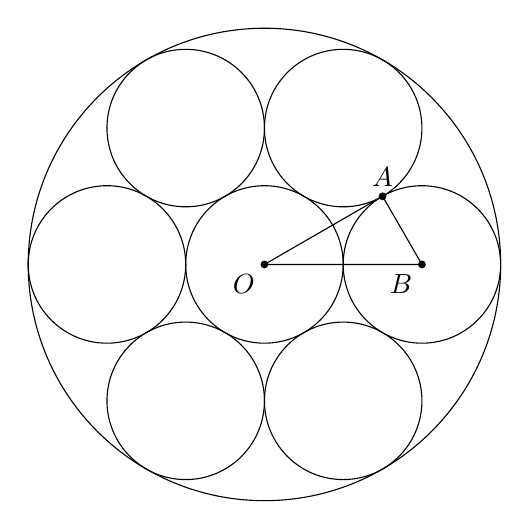
\begin{tikzpicture}
            \draw (0, 0) circle(3);
            \draw (0, 0) circle(1);

            \foreach \i in {0, 1, 2, 3, 4, 5} {
                \draw ({2 * cos(180 * \i / 3)}, {2 * sin(180 * \i / 3)}) circle(1);
            }

            \fill ({sqrt(3) * cos(30)}, {sqrt(3) * sin(30)}) circle(0.05);
            \fill (0, 0) circle(0.05);
            \fill (2, 0) circle(0.05);

            \node[anchor=north east] at (0, 0) {\( O \)};
            \node[anchor=south] at ({sqrt(3) * cos(30)}, {sqrt(3) * sin(30)}) {\( A \)};
            \node[anchor=north east] at (2, 0) {\( B \)};

            \draw (0, 0) -- ({sqrt(3) * cos(30)}, {sqrt(3) * sin(30)}) -- (2, 0) -- cycle;
        \end{tikzpicture}
        \caption{The diagram for Problem 1.}
    \end{figure}
\end{solution}

\begin{chirpbox}
\begin{problemnum}
    For eaceh positive integer \( k \), let \( S_k \) denote the increasing arithmetic sequence of integers whose first term is \( 1 \) and whose common difference is \( k \). For how many values of \( k \) does \( S_k \) contain the term \( 2005 \)?
\end{problemnum}
\end{chirpbox}

\begin{solution}
    Equivalently, we want to find the number of values \( k \) such that
    \[
        2005 = 1 + k n \iff 2004 = kn
    ,\]
    for some \( n \). This is simply just the number of divisors of \( 2004 \), which is \( \boxed{012} \).
\end{solution}

\begin{chirpbox}
    \begin{problemnum}
        How many positive integers have exactly three proper divisors, each of which is less than \( 50 \)?
    \end{problemnum}
\end{chirpbox}

\begin{solution}
    Note that the number of proper divisors of a number \( n \) is simply one less than the number of divisors of \( n \). Thus, we are searching for numbers with proper divsiors less than \( 50 \) that have \( 4 \) divisors.

    Observe that the only numbers of this form are \( p^3 \) and \( pq \), where \( p \) and \( q \) are prime. Thus there are two cases that we must count:
    \begin{itemize}
        \item All numbers of the form \( p^3 \) such that \( p^2 < 50 \) and
        \item All numbers of the form \( pq \) where \( p < q < 50 \).
    \end{itemize}
    For convenience of counting, we will list out all primes less than \( 50 \):
    \[
        \textsf{primes}_{< 50} = \{2, 3, 5, 7, 11, 13, 17, 19, 23, 29, 31, 37, 41, 43, 47\}
    .\]
    The first case has only four numbers that satisfy the conditions: \( 2^3, 3^3, 5^3, 7^3 \). The second case is also rather easy to count, because we are choosing two unique primes from the list so there are
    \[
        \binom{15}{2} = 7 \cdot 15 = 105
    .\]
    This gives us a final answer of \( 4 + 105 = \boxed{109} \).
\end{solution}

\begin{chirpbox}
    \begin{problemnum}
        The director of a marching band wishes to place the members into a formation that includes all of them and has no unfilled positions. If they are arranged in a square formation, there are \( 5 \) members left over. The director realizes that if he arranges the group in a formation with \( 7 \) more rows than columns, there are no members left over. Find the maximum number of members this band can have.
    \end{problemnum}
\end{chirpbox}

\begin{solution}
    In other words, the problem statement is telling us that for some \( n,m \)
    \[
        n^2 + 5 = m(m + 7)
    ,\]
    and we must maximize this common value.

    Observe that the equation can be rewritten as
    \[
        n^2 = m^2 + 7m - 5 := M
    .\]
    We shall now use some bounding to determine the possible values of \( m \). We have that
    \begin{align*}
        (m + 3)^2 &= m^2 + 6m + 9 \\
        (m + 4)^2 &= m^2 + 8m + 16
    .\end{align*}
    We would like to bound the maximum value of \( M \) between these two square values. We can see that \( M < (m+4)^2 \) for all values of \( m \), so in theory the largest value of \( M \) must be \( (m+3)^2 \). Because \( M - (m+3)^2 = m - 14 \), we have that \( M = (m+3)^2 \) when \( m = 14 \). As a sanity check, we know that \( M < (m+3)^2 \) for \( m < 14 \) and \( (m+3)^2 < M < (m+4)^2 \) for \( m > 14 \). Thus the common value \( 14(21) = \boxed{294} \).
\end{solution}

\begin{chirpbox}
    \begin{problemnum}
        Rober has \( 4 \) indistinguishable gold coins and \( 4 \) indistinguishable silver coins. Each coin has an engraving of one face on one side, but not on the other. He wants to stack the eight coins on a talbe into a single stack so that no two adjacent coins are face to face. Find the number of possible distinguishable arrangements of the \( 8 \) coins.
    \end{problemnum}
\end{chirpbox}

\begin{solution}
    Notice that for any arrangement of coin faces in the stack, there will always be
    \[
        \binom{8}{4} = 70
    \]
    ways to assign them colors of silver and gold, so we shall for the moment only concern ourselves with counting the number of face arrangements and then multiply this factor later.

    Consider what happens when Robert places down a coin face on the stack. The following coin then must be placed face up on the stack again, as placing it face down would go against the constraints of the problem. Coins placed face down, however, may have both face up and face down coins placed on top of them. Thus each arrangement of coin faces is uniquely determined by the position of the first face up coin in the sequence. There are \( 8 \) places to put a face up coin and also \( 1 \) more arrangement that doesn't have any face up coins, so there are \( 9 \) total arrangements without considering color. This means that the answer is \( 9 \cdot 70 = 630 \).
\end{solution}

\begin{chirpbox}
    \begin{problemnum}
        Let \( P \) be the product of the nonreal roots of \( x^4 - 4x^3 + 6x^2 - 4x = 2005 \). Find \( \lfloor P \rfloor \).
    \end{problemnum}
\end{chirpbox}

\begin{solution}
    The obvious first step is to factor the polynomial. The equation given simplifies to
    \[
        (x-1)^4 = 2006
    .\]
    This has four roots, namely \(1 +  \sqrt[4]{2006} i^k \) for \( k = 0, 1, 2, 3 \), for which \( k = 1, 3 \) gives nonreal solutions. This means that
    \[
        P = \left( 1 + \sqrt[4]{2006}i \right) \left( 1 - \sqrt[4]{2006}i \right) = 1 + \sqrt{2006}
    .\]
    Since \( 44 = \sqrt{1936} < \sqrt{2006} < \sqrt{2025} = 45 \), the answer is \( 1 + 44 = \boxed{045} \).
\end{solution}

\begin{chirpbox}
    \begin{problemnum}
        In quadrilateral \( ABCD \), \( BC = 8 \), \( CD = 12 \), \( AD = 10 \), and \( \angle A = \angle B = 60^\circ \). Given that \( AB = p + \sqrt{q} \), where \( p \) and \( q \) are positive integers, find \( p + q \).
    \end{problemnum}
\end{chirpbox}

\begin{solution}
    As always, drawing a diagram helps immensely, but I'll omit one for right now. Extend perpendiculars from \( C \) and \( D \) down to \( AB \) and denote the intersection points to be \( E \) and \( F \) respectively. Additionally, from \( C \) draw the line parallel to \( AB \) and denote its intersection with \( DF  \) to be \( G \). From this, we have that \( AB = AF + EF + BE \).

    It is rather easy to obtain \( BE \) and \( AF \). By basic trigonometry, we have that
    \begin{align*}
        BE &= 8 \cos{\left( 60^\circ \right)} \\
        AF &= 10 \cos{\left( 60^\circ \right)}
    .\end{align*}
    In order to obtain \( EF \), we can realize that it is equal to \( CG \) and see that since \( CGD \) forms a right triangle, we can use the Pythagorean theorem to obtain the desired length. Since \( CD \) is given and \( DG = DE - CF = 10 \sin{\left( 60^\circ \right)} - 8 \sin{\left( 60^\circ \right)} = 2 \sin{\left( 60^\circ \right)} \), we have that
    \[
        CG = \sqrt{144 - 4 \sin^2{\left( 60^\circ \right)}} = \sqrt{141}
    .\]
    This tells us that \( AB = 9 + \sqrt{141} \), so \( p + q = \boxed{150} \).
\end{solution}

\begin{chirpbox}
    \begin{problemnum}
        The equation \( 2^{333x-2} + 2^{111x + 2} = 2^{222x+1} + 1 \) has three real roots. Given that their sum \( m / n \) where \( m \) and \( n \) are coprime positive integers, find \( m + n \).
    \end{problemnum}
\end{chirpbox}

\begin{solution}
    We make the substitution \( t = 2^{111x} \). Written the other away around, this is \( x = (\log_2{t}) / 111 \). Doing so transforms the exponential equation into the following polynomial equation:
    \[
        t^3 - 8 t^2 + 16t - 4 = 0
    .\]
    Let \( t_1, t_2, t_3 \) denote the three roots of this polynomial. Vieta's tells us that \( t_1 t_2 t_3 = 4 \), and we also have that \( t_1 t_2 t_3 = 2^{111(x_1 + x_2 + x_3)} \), where \( x_1, x_2, x_3 \) are the solutions to the original equation. This tells us that \( x_1 + x_2 + x_3 = 2 / 111 \), so the answer is \( \boxed{113} \).
\end{solution}

\setcounter{pnum}{11}

\begin{chirpbox}
    \begin{problemnum}
        For positive integers \( n \), let \( \tau (n) \) denote the number of positive integer divisors of \( n \), including \( 1 \) and \( n \). Define \( S(n) \) by \( S(n) = \tau(1) + \tau(2) + \cdots + \tau(n) \).
        
        \vspace{0.3cm}

        Let \( a \) denote the number of positive integers \( n \le 2005 \) with \( S(n) \), and let \( b \) denote the number of positive integers \( n \le 2005 \) with \( S(n) \) even. Find \( \lvert a - b \rvert \).
    \end{problemnum}
\end{chirpbox}

\begin{solution}
    Recall that for a number \( n \) with prime factorization \( p_1^{e_1} p_2^{e_2} \cdots p_k^{e_k} \) we have that
    \[
        \tau(n) = (e_1 + 1) (e_2 + 1) \cdots (e_k + 1)
    .\]
    Observe that in order for this number to be odd, each \( e_i \) must be even, which is only true if \( n \) is a perfect square. Because of this, the parity of \( S(n) \) only flips at perfect squares. Since \( S(n) \) starts out as being odd \( n = 1 \), we see that
    \begin{itemize}
        \item \( S(n) \) is odd for \( (2k - 1)^2 \le n < (2k)^2  \) and
        \item \( S(n) \) is even for \( (2k)^2 \le n < (2k + 1)^2 \).
    \end{itemize}
    Since \( 44^2 < 2005 < 45^2 \), we can rather easily evaluate \( a \) (counting for only when \( S(n) \) is odd) without having to worry about boundary conditions and simply use the fact that \( \lvert a - b \rvert = \lvert 2a - 2005 \rvert \) to determine our answer.

    Observe that
    \begin{align*}
        a &= \sum_{k = 1}^{22}  \textsf{length}\Bigl( \bigl[(2k - 1)^2, (2k)^2\bigr) \Bigr) \\
        &= \sum_{k = 1}^{22} (2k)^2 - (2k-1)^2 = \sum_{k = 1}^{22} 4k - 1 \\
        &= 2(22)(23) - 22 = 45 \cdot 22 \\
        &= 990
    .\end{align*}
    This tell us that \( \lvert a - b \rvert = 2005 - 1980 = \boxed{025} \).
\end{solution}

\begin{chirpbox}
    \begin{problemnum}
        A particle moves in the \( 2 \)D plane according to the following rules:
        \begin{enumerate}
            \item From any lattice point \( (a, b) \), the particle may only move to \( (a+1,b), (a, b+1), \) or \( (a+1,b+1) \).
            \item There are no right angle turns in the particle's path.
        \end{enumerate}
        How many different paths can the particle take from \( (0,0) \) to \( (5,5) \)?
    \end{problemnum}
\end{chirpbox}

\begin{solution}
    Suppose the particle makes \( r \) moves to the right, \( u \) moves upwards, and \( d \) moves diagonally along the path. According to the problem, we have the following relation between these values:
    \begin{align*}
        r + d &= 5 \\
        u + d &= 5
    .\end{align*}
    This tells us that \( r = u \) and \( d = 5 - r = 5 - u \). Using this, we are motivated to look at the paths taken by the particle as strings. Let \( R, U, D \) represent moving to the right, up, and diagonally respectively in the path string. The second condition in the problem tells us that the string must not contain the substring \( RU \) or \( UR \). Keeping this in mind, we may do casework on these path strings.
    \begin{itemize}
        \item Case  \( r = u = 0 \). This tells us that \( d = 5 \), so there is \( 1 \) path.
        \item Case \( r = u = 1 \), \( d = 4 \).
    \end{itemize}
\end{solution}

\end{document}
